\begin{ledgroupsized}[r]{120mm}
\footnotesize 
\pstart 
\noindent\textbf{\"{U}berlieferung:}
\pend
\end{ledgroupsized}

\begin{ledgroupsized}[r]{114mm}
\footnotesize 
\pstart \parindent -6mm
\makebox[6mm][l]{\textit{LiH}}%
Anstreichungen und Anmerkungen in \textsc{I. G. Pardies}, \textit{La statique ou la science des forces mouvantes},\cite{00296} Paris 1673: \textsc{Hannover}, GWLB, Leibn. Marg. 66.
\pend
\end{ledgroupsized}
 %\normalsize
\vspace*{5mm}
\begin{ledgroup}
\footnotesize 
\pstart
\noindent\footnotesize{\textbf{Datierungsgr\"{u}nde:} Die Marginalien in diesem Exemplar von Pardies' \textit{La statique}\cite{00296} sind wahr\-schein\-lich in Zusammenhang mit N.~7, % = LH035_14_02_128v.tex + LH035_14_02_127r.tex = Aus und zu I. G. Pardies, La statique
d.h. mit Leibniz' Auszügen aus derselben Abhandlung, verfasst worden.
Die editorisch erschlossene Datierung von N.~7 -- Mai 1673 -- wird daher auch für N.~44 übernommen.}
\pend
\end{ledgroup}

\vspace{8mm}
\pstart 
\normalsize
\noindent [p. 112] 
\pend
%\vspace{1em}
\pstart
\centering                    
\noindent 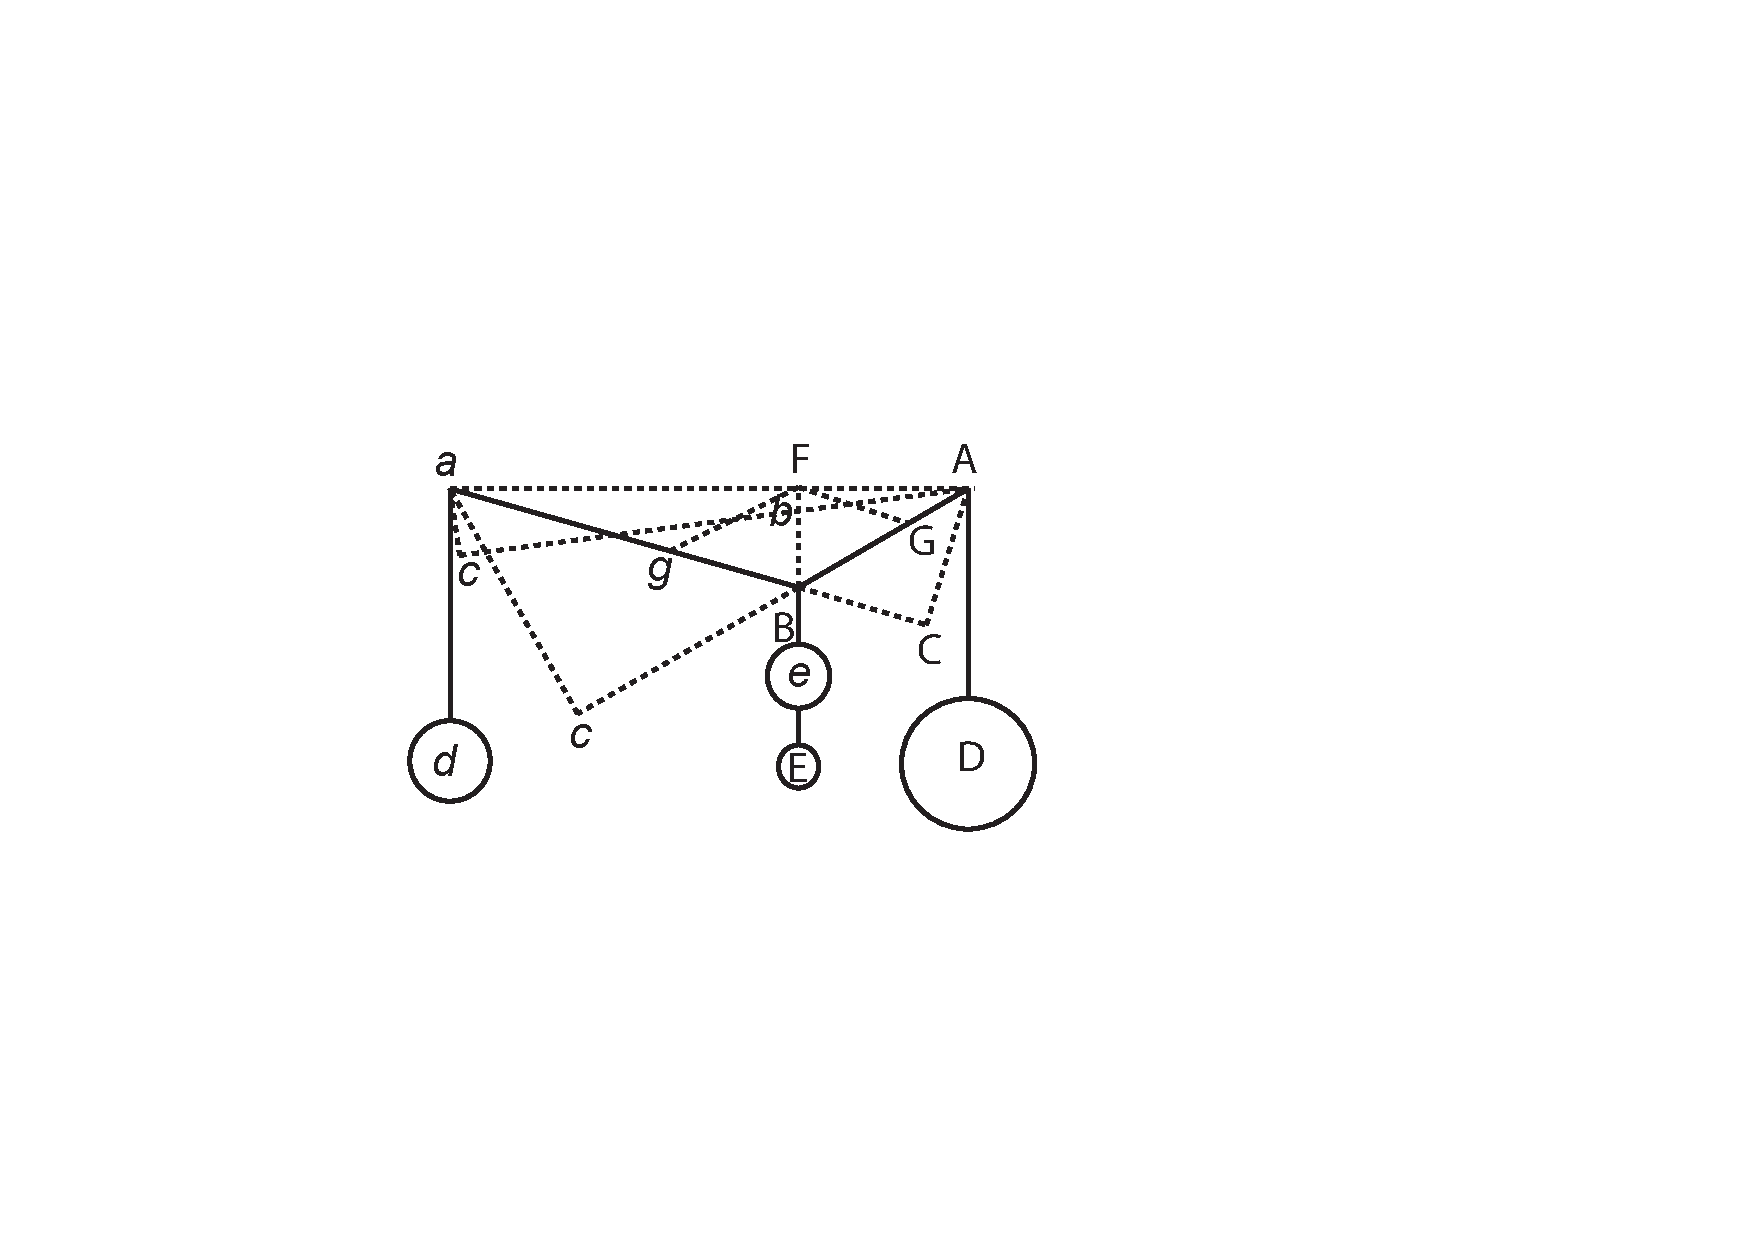
\includegraphics[width=0.45\textwidth]{images/pardies1673-d1.pdf}\\
              \noindent \centering [\textit{Fig. 1}] 
\pend
\vspace{1em}
\count\Afootins=1000
\pstart Pour \setline{8}le prouver, imaginons que les lignes \textit{AC},\edtext{}{\lemma{}\Afootnote{\textit{Am unteren Rand unter Text und Zeichnung}: Si alligata sit chorda in \textit{A}, et una sit trochlea \textit{a}, et agit pondus unum ut \textit{D}, videndum an non sit idem ac si duae essent trochleae duaque pondera aequalia.\vspace{2mm}}} [p. 113] \textit{a c} tombent perpendiculairement sur les cordes \textit{aBC}, \textit{ABc}, prolong\'{e}es s'il en est besoin.
\pend 
\pstart 
[p. 122] Je ne m'arreste pas \`{a} prouver que ces cordes (lors qu'elles ne sont pas paralleles) se doivent croiser en quelque point; car il est assez manifeste que les points \textit{a A} , \textit{o n} sont en mesme \edtext{plan.}{\lemma{}\Afootnote{\textit{Leibniz unterstreicht}: plan. \textit{und schreibt daneben}: rien n'emp\^{e}che qu'on ne les fasse tomber en deux plans differens.}}
\pend
\count\Afootins=1500
 

